\documentclass[lettersize, journal]{IEEEtran}
\usepackage[utf8]{inputenc} 
\usepackage[T1]{fontenc}   
\usepackage{mathptmx}       
\usepackage{graphicx}      
\usepackage{float}          
\usepackage{algorithmic}
\usepackage{algorithm}
\usepackage{caption}        
\usepackage{subcaption}     
\usepackage{biblatex}       
\usepackage{amsmath, amsfonts, amssymb}  
\usepackage{hyperref}
\usepackage{enumitem}       
\usepackage{tikz, pgfplots}
\usetikzlibrary{shapes,arrows.meta, positioning}

\addbibresource{reference.bib} 



\begin{document}

% Paper title
\title{Forecasting Hospitalization Demand in England during COVID-19 Pandemic: A Mathematical Modeling Approach}
\author{Michael Ajao-olarinoye}

\maketitle
% \thispagestyle{empty}


\begin{abstract}

\end{abstract}

\begin{IEEEkeywords}

\end{IEEEkeywords}

\section{Introduction}
\IEEEPARstart{T}{his} paper delves into the mathematical modeling of infectious diseases, specifically focusing on the COVID-19 pandemic. The primary objective is to understand the dynamics of COVID-19 transmission and to forecast the demand for mechanical ventilators in England, a critical healthcare resource during the peaks of the pandemic.

\section{Problem Statement}
The outbreak of the COVID-19 pandemic has posed significant challenges to healthcare systems worldwide. One of the major concerns during the pandemic's peaks has been the potential overwhelming demand on healthcare resources, particularly the demand for intensive care units (ICUs) and mechanical ventilators. This study aims to develop a mathematical model to understand the dynamics of COVID-19 transmission and forecast the demand for mechanical ventilators in England.

\section{Model Assumptions}
\begin{enumerate}
    \item The population is constant, i.e., no births or non-COVID-related deaths are considered.
    \item The disease transmission occurs only between the susceptible and the infected (both asymptomatic and symptomatic) individuals.
    \item Individuals progress from being exposed to the virus to being infected (either asymptomatic or symptomatic).
    \item Symptomatic infected individuals may require mechanical ventilation if their condition deteriorates.
    \item Ventilated patients either recover or die.
    \item Recovered individuals can lose immunity and become susceptible again.
\end{enumerate}

\section{Model Definition}
\subsection{Compartments}
\begin{itemize}
    \item \( S(t) \): Susceptible individuals at time \( t \).
    \item \( E(t) \): Exposed individuals at time \( t \).
    \item \( I_a(t) \): Asymptomatic infected individuals at time \( t \).
    \item \( I_s(t) \): Symptomatic infected individuals at time \( t \).
    \item \( V(t) \): Individuals on ventilators at time \( t \).
    \item \( R(t) \): Recovered individuals at time \( t \).
    \item \( D(t) \): Deceased individuals at time \( t \).
\end{itemize}

\subsection{Differential Equations}
\begin{align*}
    \frac{dS}{dt}   & = -\beta S (I_a + I_s) + \omega R                              \\
    \frac{dE}{dt}   & = \beta S (I_a + I_s) - \sigma E                               \\
    \frac{dI_a}{dt} & = p \sigma E - \gamma_a I_a                                    \\
    \frac{dI_s}{dt} & = (1-p) \sigma E - \gamma_s I_s - \rho I_s                     \\
    \frac{dV}{dt}   & = \rho I_s - (\nu + \alpha) V                                  \\
    \frac{dR}{dt}   & = \gamma_a I_a + \gamma_s I_s + (1-\delta) \alpha V - \omega R \\
    \frac{dD}{dt}   & = \delta \alpha V + \nu V
\end{align*}

\subsection{Parameters}
\begin{itemize}
    \item \( \beta \): Transmission rate.
    \item \( \sigma \): Rate of progression from exposed to infected.
    \item \( \gamma_a \): Recovery rate for asymptomatic individuals.
    \item \( \gamma_s \): Recovery rate for symptomatic individuals.
    \item \( \rho \): Rate at which symptomatic individuals require ventilation.
    \item \( \alpha \): Recovery rate for ventilated individuals.
    \item \( \nu \): Death rate for individuals on ventilators.
    \item \( \delta \): Proportion of ventilated patients who die.
    \item \( \omega \): Rate at which recovered individuals lose immunity.
    \item \( p \): Proportion of exposed individuals who become asymptomatic infected.
\end{itemize}

\begin{figure}[h]
    \centering
    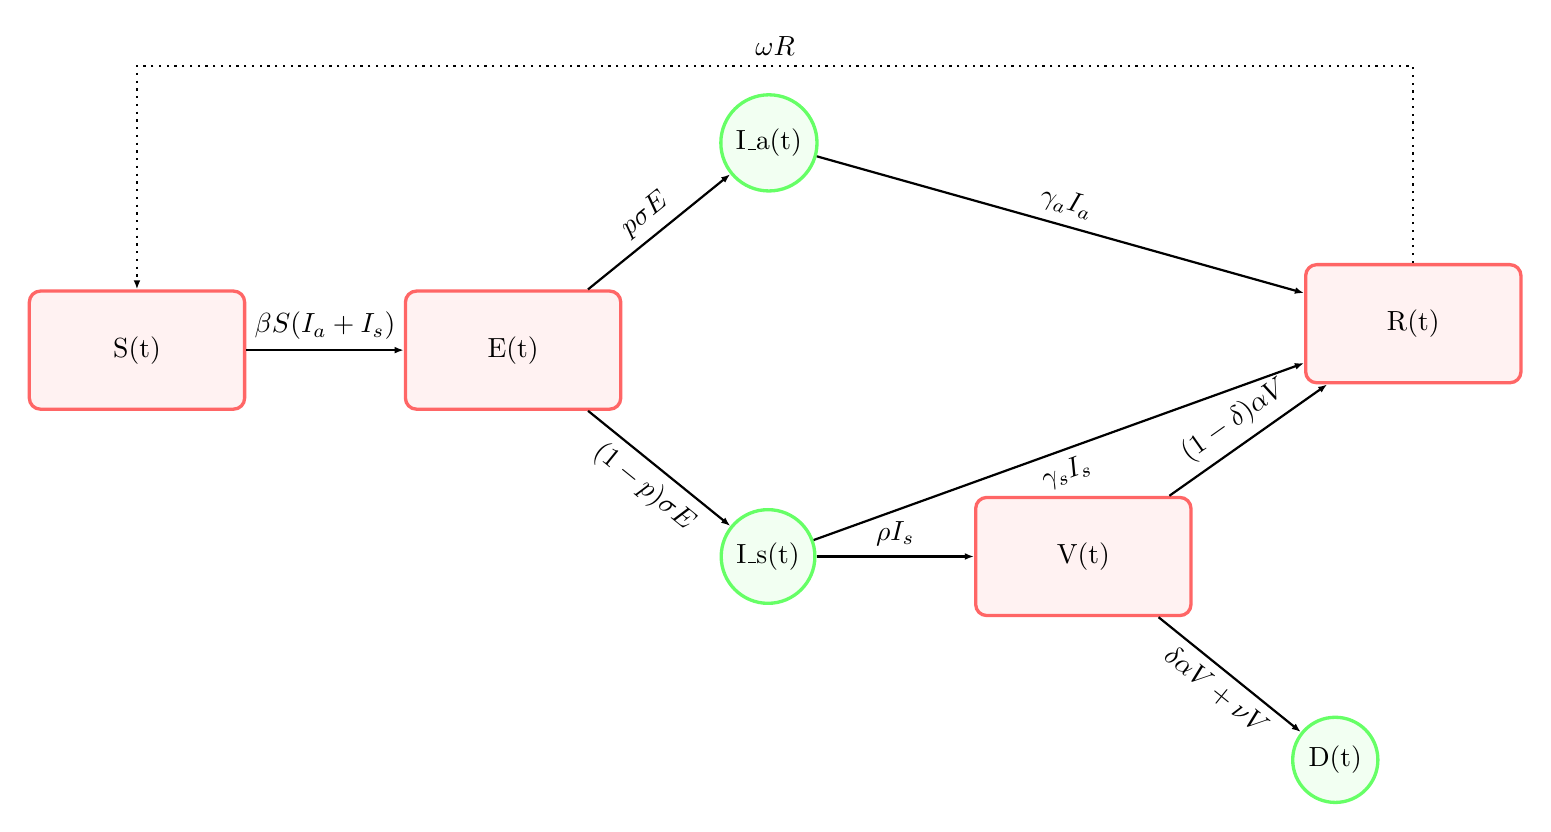
\begin{tikzpicture}[node distance=2.0cm, thick]
        % Define block styles
        \tikzstyle{roundnode} = [circle, draw=green!60, fill=green!5, very thick, minimum size=1cm, text centered]
        \tikzstyle{squarednode} = [rectangle, draw=red!60, fill=red!5, very thick, text width=2.5cm, text centered, rounded corners, minimum height=1.5cm]
        \tikzstyle{line} = [draw, -{Latex[scale=0.5]}]

        % Define nodes
        \node [squarednode] (S) {S(t)};
        \node [squarednode, right=of S] (E) {E(t)};
        \node [roundnode, above right=of E] (Ia) {I\_a(t)};
        \node [roundnode, below right=of E] (Is) {I\_s(t)};
        \node [squarednode, right=of Is] (V) {V(t)};
        \node [squarednode, above right=of V] (R) {R(t)};
        \node [roundnode, below right=of V] (D) {D(t)};

        % Connect nodes with paths
        \draw[line] (S) -- node[midway, above] { \( \beta S (I_a + I_s) \) } (E);
        \draw[line] (E) -- node[midway, sloped, above] { \( p \sigma E \) } (Ia);
        \draw[line] (E) -- node[midway, sloped, below] { \( (1-p) \sigma E \) } (Is);
        \draw[line] (Is) -- node[midway, above] { \( \rho I_s \) } (V);
        \draw[line] (Ia) -- node[midway, sloped, above] { \( \gamma_a I_a \) } (R);
        \draw[line] (Is) -- node[midway, sloped, below] { \( \gamma_s I_s \) } (R);
        \draw[line] (V) -- node[midway, sloped, above] { \( (1-\delta) \alpha V \) } (R);
        \draw[line] (V) -- node[midway, sloped, below] { \( \delta \alpha V + \nu V \) } (D);
        \draw[line, dotted] (R.north) -- ++(0,2.5cm) -| node[pos=0.25, above] { \( \omega R \) } (S.north);

    \end{tikzpicture}
    \caption{Compartmental flow of the COVID-19 Transmission Dynamics Model.}
\end{figure}

\section{Mathematical Proof of the Model}
The model is a system of ordinary differential equations (ODEs) derived from the law of mass action. The sum of all compartments at any time \( t \) is equal to the constant population \( N \), ensuring the conservation of mass:

\[ S(t) + E(t) + I_a(t) + I_s(t) + V(t) + R(t) + D(t) = N \]

The non-negativity of the solutions is ensured by the non-negative initial conditions and the structure of the ODEs, which prevents negative values in any compartment.

\section{Reproduction Numbers for the Epidemic Model}
In this section, we derive the basic reproduction number \( R_0 \) and the effective reproduction number \( R_t \) using the Next-Generation Matrix (NGM) method.

\subsection{Basic Reproduction Number \( R_0 \)}
The basic reproduction number, \( R_0 \), represents the average number of secondary infections produced by a single infected individual in a completely susceptible population. Using the NGM method, \( R_0 \) is derived as:

\[ R_0 = \frac{\beta N ( \rho - \sigma + p \sigma + \gamma_s )}{p \sigma ( \rho + \gamma_s )} \]

\subsection{Effective Reproduction Number \( R_t \)}
The effective reproduction number, \( R_t \), represents the average number of secondary infections produced by one infected individual at time \( t \) in a population that is not entirely susceptible. It is formulated as:

\[ R_t = \frac{\beta S(t) ( \rho - \sigma + p \sigma + \gamma_s )}{p \sigma ( \rho + \gamma_s )} \]

\section{Real-World Application}
This model serves as a tool for understanding and predicting the demand for critical healthcare resources




\end{document}